\documentclass[11pt]{article}

%  USE PACKAGES  ---------------------- 
\usepackage[margin=0.7in,vmargin=1in]{geometry}
\usepackage{amsmath,amsthm,amsfonts}
\usepackage{amssymb}
\usepackage{fancyhdr}
\usepackage{enumerate}
\usepackage{mathtools}
\usepackage{multirow}
\usepackage{array}
\usepackage{hyperref,color}
\usepackage{enumitem,amssymb}
\newlist{todolist}{itemize}{4}
\setlist[todolist]{label=$\square$}
\usepackage{pifont}
\newcommand{\cmark}{\ding{51}}%
\newcommand{\xmark}{\ding{55}}%
\newcommand{\done}{\rlap{$\square$}{\raisebox{2pt}{\large\hspace{1pt}\cmark}}%
\hspace{-2.5pt}}
\newcommand{\HREF}[2]{\href{#1}{#2}}
\usepackage{textcomp}
\usepackage{listings}
\lstset{
basicstyle=\small\ttfamily,
% columns=flexible,
upquote=true,
breaklines=true,
showstringspaces=false
}
%  -------------------------------------------- 

%  HEADER AND FOOTER (DO NOT EDIT) ----------------------
\newcommand{\problemnumber}{0}
\pagestyle{fancy}
\fancyhead{}
\fancyfoot[L]{IE 332}
\fancyfoot[C]{Project submission}
\fancyfoot[R]{Page \thepage}
\renewcommand{\footrulewidth}{0.4pt}

%  --------------------------------------------


%  COVER SHEET (FILL IN THE TABLE AS INSTRUCTED IN THE ASSIGNMENT) ----------------------
\newcommand{\addcoversheet}{
\clearpage
\thispagestyle{empty}
\vspace*{0.5in}

\begin{center}
\Huge{{\bf IE332 Project \#2}} % <-- replace with correct assignment #

Due: April 28th, 11:59pm EST % <-- replace with correct due date and time
\end{center}

\vspace{0.3in}

\noindent We have {\bf read and understood the assignment instructions}. We certify that the submitted work does not violate any academic misconduct rules, and that it is solely our own work. By listing our names below we acknowledge that any misconduct will result in appropriate consequences. 

\vspace{0.2in}

\noindent {\em ``As a Boilermaker pursuing academic excellence, I pledge to be honest and true in all that I do.
Accountable together -- we are Purdue.''}

\vspace{0.3in}

\begin{table}[h!]
  \begin{center}
    \label{tab:table1}
    \begin{tabular}{c|m{5em}m{5em}m{5em}m{5em}m{4em}|c|c}
      Student & Algorithm Development & Complexity Analysis & Implemen-tation & Performance Analysis/Testing & Report & Overall & DIFF\\
      \hline
      Gabi & x & x & x & x & x & x& x\\
      Haley & x & x & x & x & x & x & x\\
      Declan & x & x & x & x & x & x & x\\
      Ben & x & x & x & x & x & x & x\\
      Rohan & x & x & x & x & x & x & x\\
      \hline
      St Dev & x & x & x & x & x & x & x
    \end{tabular}
  \end{center}
\end{table}

\vspace{0.2in}

\noindent Date: \today.
}
%  -----------------------------------------

%  TODO LIST (COMPLETE THE FULL CHECKLIST - USE AS EXAMPLE THE FIRST CHECKED BOXES!) ----------------------
\newcommand{\addtodo}{
\clearpage
\thispagestyle{empty}

\section*{Read Carefully. Important!}

\noindent By electronically uploading this assignment to Brightspace you acknowledge these statements and accept any repercussions if in any violation of ANY Purdue Academic Misconduct policies. You must upload your homework on time for it to be graded. No late assignments will be accepted. {\bf Only the last uploaded version of your assignment before the due date will be graded}.

\vspace{0.2in}

\noindent {\bf NOTE:} You should aim to submit no later than 30 minutes before the deadline, as there could be last minute network traffic that would cause your assignment to be late, resulting in a grade of zero. 

\vspace{0.2in}

\noindent When submitting your assignment it is assumed that every student considers the below checklist, as there are grading consequences otherwise (e.g., not submitting a cover sheet is an automatic grade of ZERO).

\begin{todolist}

    \item[\done] Your solutions were prepared using the \LaTeX template provided in Brightspace. 
    \item[\done] Your submission has a cover sheet as its first page and this checklist as its second page, according to the template provided.
	 \item[\done] All of your solutions (program code, etc.) are included in the submission as requested. % Check this checkbox and the following ones if satisfied <---
    \item[\done] You have not included any screen shots, photos, etc. (plots should be intermediately saved as .png files and then added into your .tex file). % <---
	 \item[\done] All math notation and algorithms (algorithmic environment) are created using appropriate \LaTeX code (no pictures, handwritten solutions, etc.). % <---
    \item[\done] The .pdf is submitted as an individual file and not in a {\tt .zip}.
    \item[\done] You kept the \LaTeX source code in your files until this assignment is graded, in case you are required to show proof of creating your assignment using \LaTeX.  % <---
    \item[\done] If submitting with a partner, your partner is added in the submission section in Gradescope after you upload your file. % <---
    \item[\done] You have correctly matched each question to its page \# in the .pdf submission in the Gradescope section (after you uploaded your file).
    \item[\done] Watch videos on creating pseudocode if you need a refresher or quick reference to the idea. These are good starter videos:    % <---
    
     \HREF{https://www.youtube.com/watch?v=4jLO0vXPktU}{www.youtube.com/watch?v=4jLO0vXPktU} 
    
    \HREF{https://www.youtube.com/watch?v=yGvfltxHKUU}{www.youtube.com/watch?v=yGvfltxHKUU}
\end{todolist}
}

%% LaTeX
% Für alle, die die Schönheit von Wissenschaft anderen zeigen wollen
% For anyone who wants to show the beauty of science to others

%  -----------------------------------------


\begin{document}
\addcoversheet
\addtodo
\pagebreak
\tableofcontents
\pagebreak

% BEGIN YOUR ASSIGNMENT HERE:
\def\Plus{\texttt{+}}
\section{Introduction}
\underline{Github Link:}\\

\subsection{Executive Summary}
\noindent This report details Team 4's efforts toward the completion of IE332's Project 2. The team attempted to complete this machine learning program through a five-subsection algorithm that fools an image classifier while following the given constraints. 

\subsection{Problem Statement}
\noindent Project 2 presented the team with a problem regarding a binary image classifier. The team is responsible for building and manipulating a majority voting classifier that weights the use of five sub-algorithms that must perform adversarial attacks on the given classifier. The purpose of these attacks is to trick the classifier into incorrectly classifying images. the team must complete this task in under ten seconds per image and without changing the input images enough that the naked eye would notice a difference.

\subsection{Sub-algorithm Introduction}

\noindent In our algorithm, we selected five sub-algorithms that will perform adversarial attacks collectively to trick the binary image classifier. After intensive research, we selected the Genetic Algorithm (GA), Particle Swarm Optimization (PSO), Simulated Annealing (SA), Hill Climbing, and Fast Gradient Sign Method (FGSM) as our algorithms to attack the classifier. 
\newline\\
\noindent The Genetic Algorithm is a heuristic that is based on natural selection where the fittest individuals are selected to pass on characteristics to the next generation (Mallawaarachchi, 2020). We selected this algorithm because of its ability to generate a variety of attacks through random mutation and its adaptability to changes in the original machine learning model. 
\newline\\
\noindent Particle Swarm Optimization implements the idea of when animals travel in a group they can profit from the experience of all other members (Tam, 2021). In terms of optimization, we start with a bunch of random points (particles) and let them look for an extremum in all directions. As the particles find extrema, they iterate and look for the next possible extrema. We selected this algorithm because it finds a solution quickly and works on a diverse set of problem types. 
\newline\\
\noindent Simulated Annealing is a stochastic global search algorithm. We selected this algorithm because of how good it is at finding a global optimum even in complex problems (Brownlee, 2021). Because particle swarm optimization may find more local optima, the team decided to alleviate this weak point by implementing simulated annealing. 
\newline\\
\noindent Hill climbing is an adversarial attack that capitalizes on the weakest points in the input data by iterating the mistake over and over again until the classifier cannot classify it anymore. The team selected this algorithm because of how easily and quickly this method can be implemented to cause damage. 
\newline\\
\noindent The final algorithm the team utilized is Fast Gradient Sign Method, which is an adversarial attack that stretches a weak point in the input data to confuse a classifier. This algorithm was implemented because of its simplicity in only needing to be run once forward and backward through the model.
\newline\\
\noindent Sub-algorithms we also looked includes the DeepFool algorithm, Gradient Descent, Broyden-Flectcher-Goldfard-Shanno (L-BFGS) algorithm and Carlini and Wasgner (CW) attack algorithm. While all are effective at adversarial attacks with extensive research to back them, they did not end up in our final algorithm. The main reason for that is the failure to implement. Either the conversion to R was too complicated or the classifier could still recognize the image at a higher than 50\% accuracy. Gradient Descent is another algorithm we looked to implement; however, it did not have an R library.   

\section{Majority Voting Classifier Design}

\noindent All experimental variants of your
algorithm (e.g. with different sub-algorithms, and so forth) should be tracked with separate branches and the best
one should then be merged into main.

\subsection{Genetic Algorithm}
\noindent Genetic Algorithm is an adversarial attack method that tricks a classifier by mutating input data. 
In our case, it does this by determining how good each pixel in the picture is, keeping the top pixels, then randomly mutating some proportion of the pixels. The algorithm repeats these steps until enough noise is generated to fool the classifier. 
\newline\\
\noindent The team decided to use the Genetic Algorithm because of how well it works with images specifically. After researching the benefits and disadvantages of Genetic Algorithm, we found a study performed by researchers from the University of Maribor, in which they applied this algorithm that created noise to images to fool an image classifier. The output images appeared to have minimal changes to the naked eye, while still containing noise and not passing the classifier's test (Rok Kukovec et al., 2021). This visual proof of image manipulation while still being successful allowed the group to feel confident in our decision to include this algorithm type in our project.

\subsection{Particle Swarm Optimization}
\noindent Particle Swarm Optimization is a population-based algorithm that focuses on finding local optima to perform an adversarial attack(Wang et al., n.d.). The basic steps of the attack are: randomly disperse particles onto the pixels of an image, change the pixel where a particle lands, find a more optimal pixel location, and move toward it. The process repeats as the particles move to an area of the image that, if altered, would maximize the probability of tricking the classifier (Tam, 2021). Toward the end of the algorithm, the swarm of particles comes together to the optimal location, similar to a flock of birds.
\newline\\
\noindent The team decided to utilize Particle Swarm Optimization because of how quickly the algorithm is at finding a solution. According to project guidelines, the classifier must the fooled in less than ten seconds per image. Therefore, as a team, we decided to focus some algorithms on speed and some on accuracy, with the weighted combination optimizing the usage of both. PSO will speed up our overall average run time, while also retaining a good solution.

\subsection{Simulated Annealing}
\noindent Simulated Annealing is a heuristic algorithm that can be used to trick an image classifier through making small changes to the original image. If the new image fools the classifier, this iteration is kept as the new original and another change is made to increase the inaccuracy of the classifier. If the new image does not fool the classifier, a different aspect of the image is changed and the iteration is repeated. Once the attack has maximized its changes to the picture to trick the classifier, while also making sure the image is still similar enough to the original that the naked eye would not notice, the algorithm stops.
\newline\\
\noindent The team decided to use simulated annealing in our main algorithm because of it's ability to avoid noise and find a global optimum. A sub-algorithm focused on finding the best possible solution is important in developing a weighted program that breaks an image classifier with optimal speed and accuracy.

\subsection{Hill Climbing}
\noindent A team of researchers might use the hill-climbing algorithm in R to complete a project that helps change the pixels from a preexisting image into a new image because it is a heuristic search algorithm that is well-suited for optimization problems like image processing. Hill-climbing algorithm starts with an initial solution and iteratively explores its neighboring solutions, selecting the one that improves the objective function. In image processing, the objective function can be the similarity measure between the original image and the modified image. By using the hill-climbing algorithm, the researchers can efficiently find the optimal set of pixel values that create a new image with desired features, such as increased contrast or reduced noise.
\newline\\
\noindent In R, we used the hill climbing algorithm can be implemented efficiently using matrix operations and vectorization. This makes it fast and scalable for processing large images. Additionally, since R provides many libraries and functions for image processing, it made it easy for us to integrate the hill climbing algorithm into a larger workflow. Overall, using the hill climbing algorithm in R can be a powerful tool for improving image quality.

\subsection{Fast Gradient Sign Method}
\noindent Fast Gradient Sign Method is a type of adversarial attack that works well with data that clusters and has a decision boundary that classifies between images (Tsui, 2018). This algorithm works by implementing noise to the input picture on the same gradient that the boundary line lies on. The loss function is calculated to find the direction in which the maximum loss will occur. Next, noise is injected to change pixels in that direction (Ansah, 2022). The purpose of the noise is to push the image classification over the decision boundary and into the cluster of opposite classifications in order to fool the classifier. 
\newline\\
\noindent Our group decided to choose FGSM because of how fast and easy it is to implement. This algorithm exploits the weaknesses of images that the image classifier cannot classify with high accuracy. Fast gradient sign method is also applicable to a wide variety of pictures so that many images could be used to test the accuracy of this adversarial attack.

\subsection{Combination of Sub-Algorithms and Weighting}



%APPENDICES
\newpage
\section{Appendices}
\subsection{Testing, Correctness, and Verification}
\subsubsection{Testing}
When evaluating the effectiveness of our adversarial attack algorithms on the neural network, we looked at the accuracy and robustness. Other testing metrics include perturbation size and transferability; however, we did not have the ability to generate additional neural networks nor other adversarial examples. Accuracy is the percentage of correctly classified examples in the test set. We dictated the last 6 images in the provided dandelion and grass image folders to be our test sets. Robustness is the ability of the model to resist adversarial attacks. This metric can be found by comparing the accuracy of the model on the original test set with the accuracy on the model with the adversarially altered test set. The tables on the next page displays a summary of the test cases for before and after the adversarial attacks are implemented. The first table displays the last 6 images for the grass model with the accuracy for before and after. The following table displays the last 6 images for the dandelion with the same information. \\


\begin{center}
\begin{tabular}{|m{5em}|m{8em}|m{11em}|m{11em}|}
\hline
Type & Image & Accuracy Before Attacks & Accuracy After Attacks \\
\hline
\multirow{6}{4em}{Grass} & 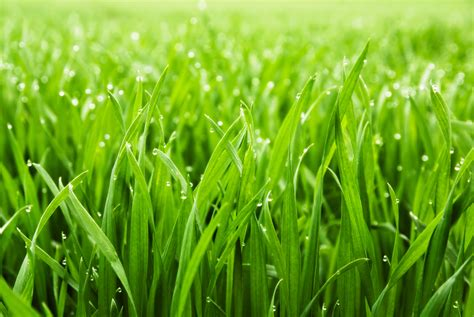
\includegraphics[width=30mm, height=15mm]{images/th-246163958.jpg} & 0.9964305 & xx \\ 
& 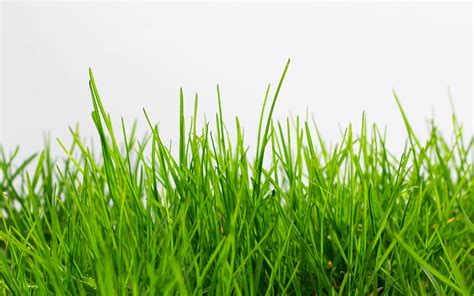
\includegraphics[width=30mm, height=15mm]{images/th-373883262.jpg} & 0.9906991 & xx \\ 
& 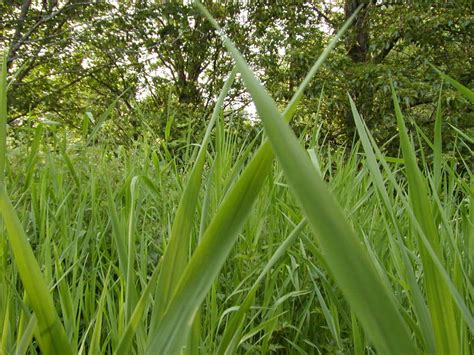
\includegraphics[width=30mm, height=15mm]{images/th-384947726.jpg} & 0.9962944 & xx \\
& 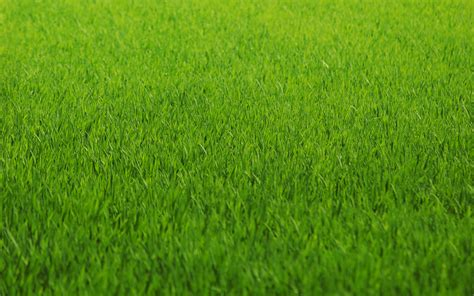
\includegraphics[width=30mm, height=15mm]{images/th-4166387598.jpg} & 0.9992237 & xx \\ 
& 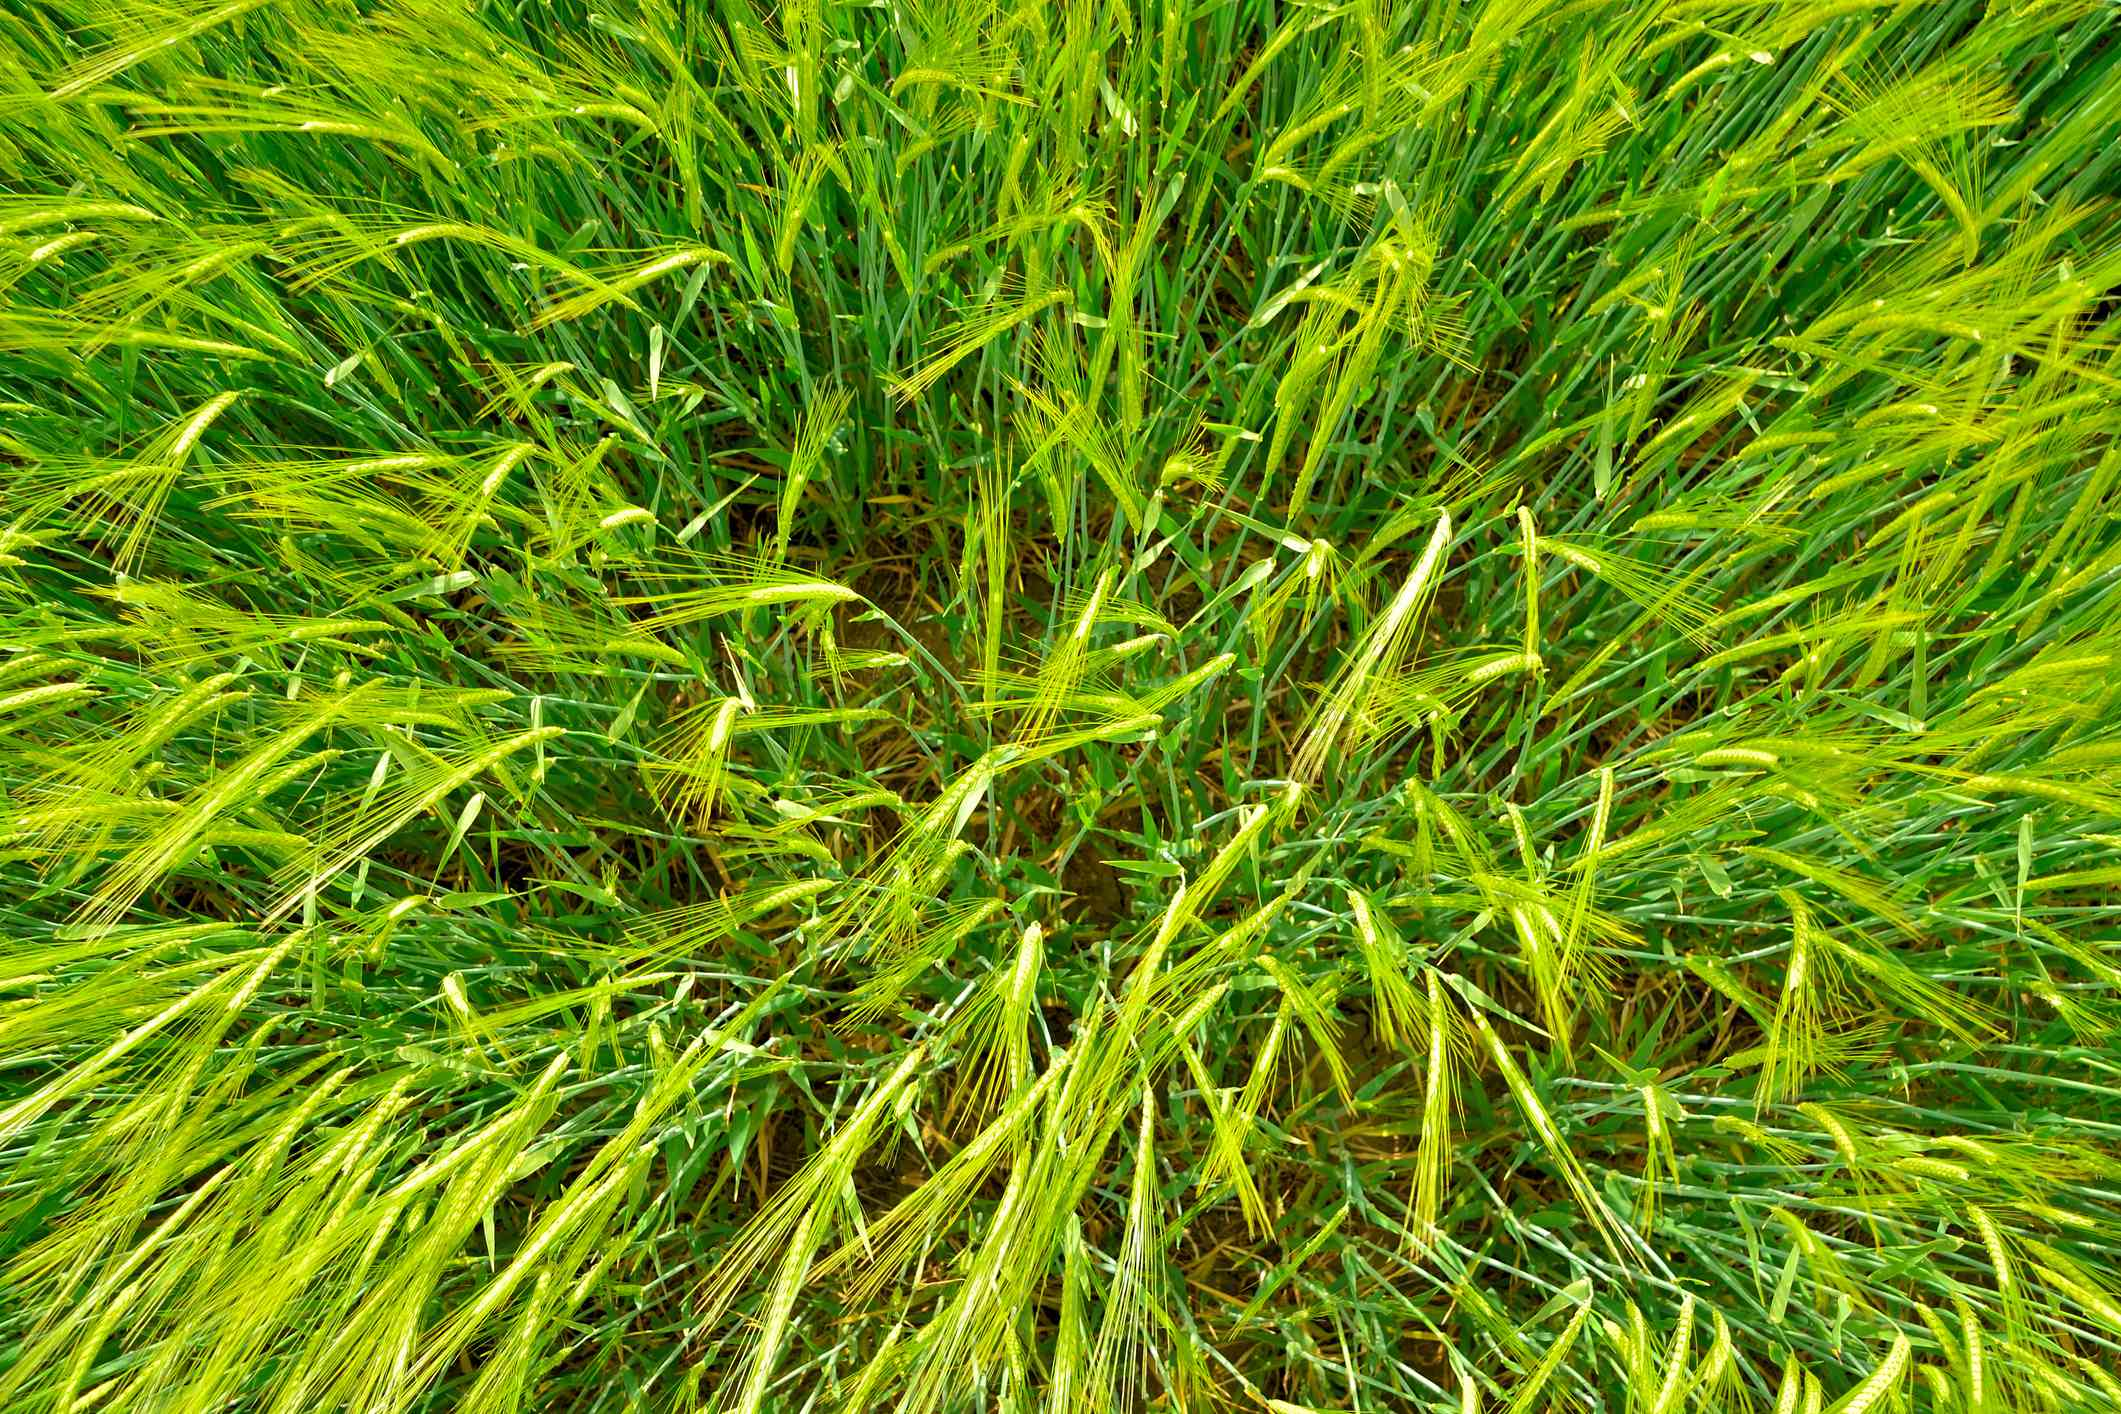
\includegraphics[width=30mm, height=15mm]{images/wheatgrass-2be8422b0eea4c969351410093ccae42-2419490567.jpg} & 0.9787846 & xx \\ 
& 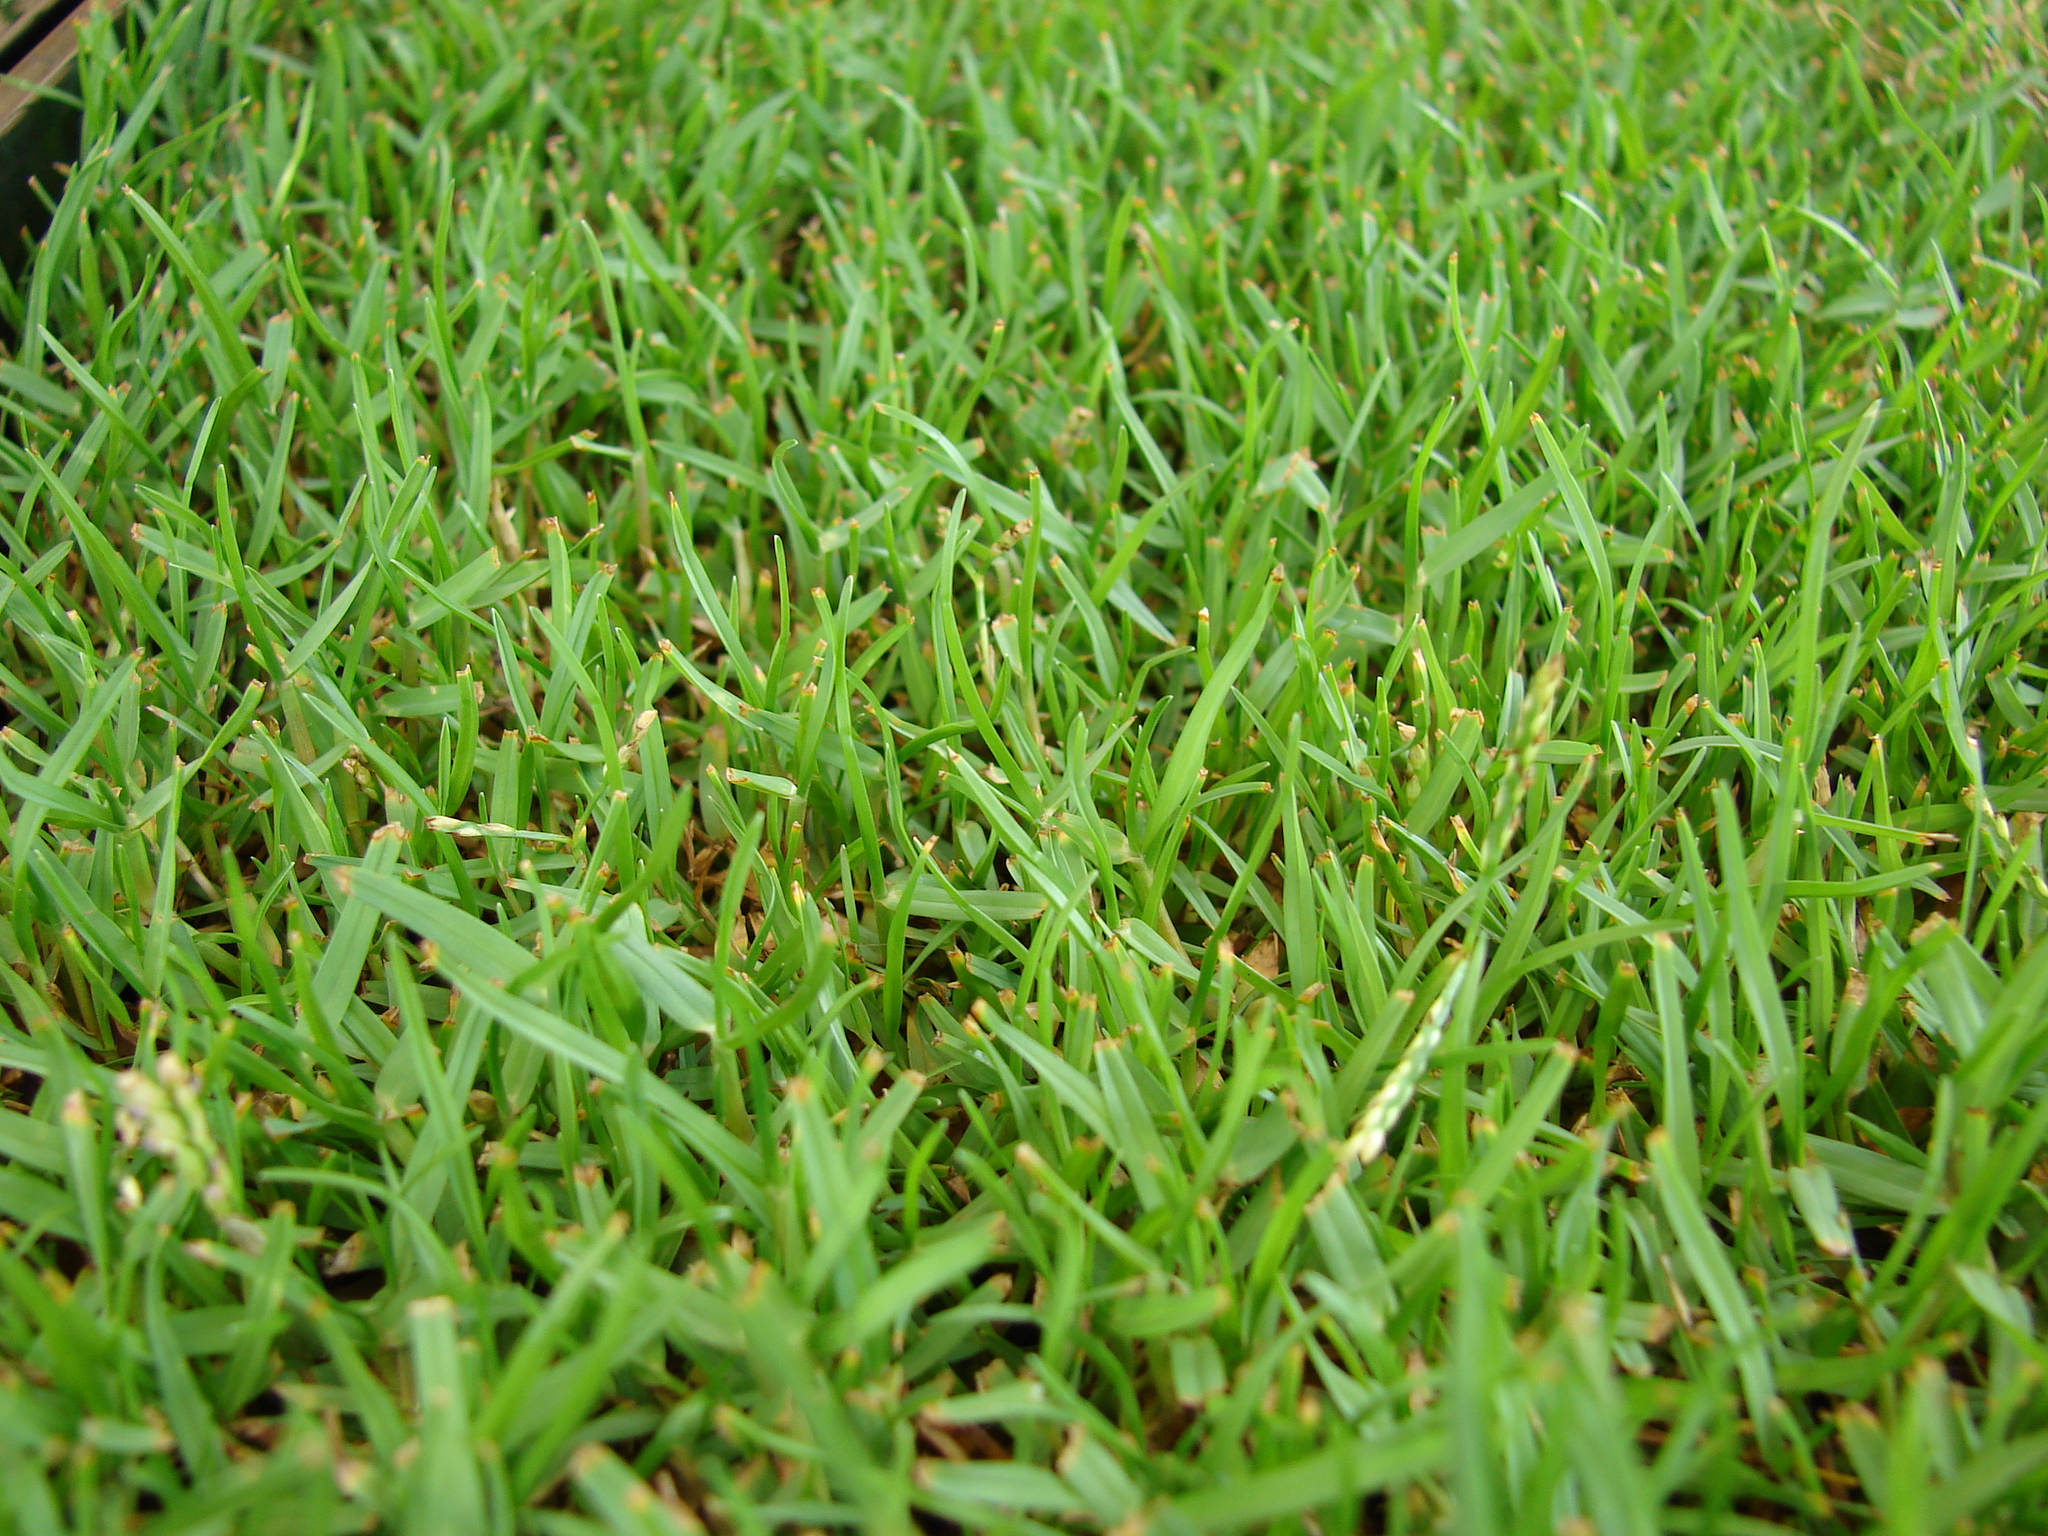
\includegraphics[width=30mm, height=15mm]{images/zoysia-grass-2723693948.jpg} & 0.9982908 & xx \\ 
\hline
\end{tabular}
\end{center}
\begin{center}
Table 1. Grass Image Accuracy Before and After Attacks
\end{center}

\begin{center}
\begin{tabular}{|m{7em}|m{8em}|m{11em}|m{11em}|}
\hline
Type & Image & Accuracy Before Attacks & Accuracy After Attacks \\
\hline
\multirow{6}{4em}{Dandelion} & 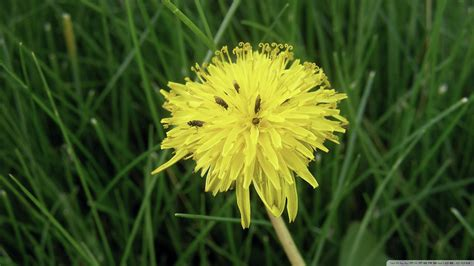
\includegraphics[width=30mm, height=15mm]{images/th-3423486846.jpg} & 0.9880867 & xx \\ 
& 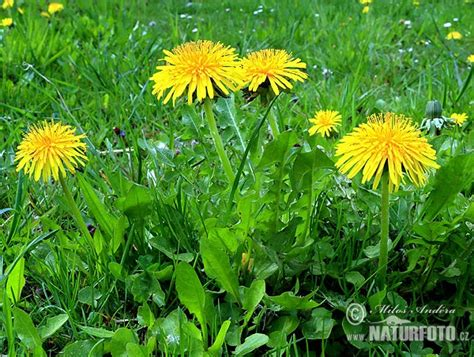
\includegraphics[width=30mm, height=15mm]{images/th-3992465304.jpg} & 0.9602737 & xx \\ 
& 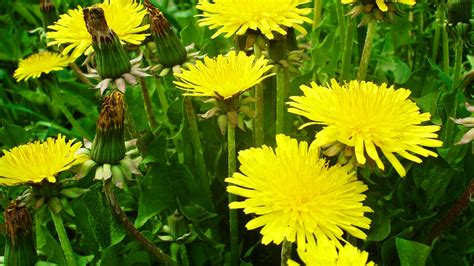
\includegraphics[width=30mm, height=15mm]{images/th-4103160292.jpg} & 0.9976503 & xx \\
& 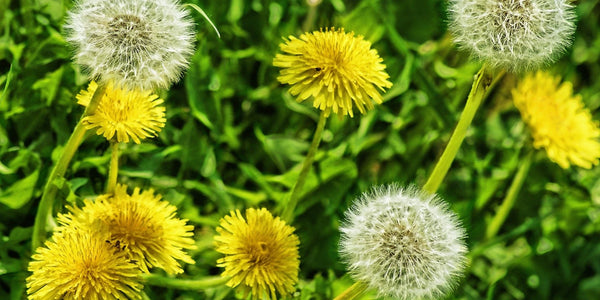
\includegraphics[width=30mm, height=15mm]{images/Types_of_Dandelion_600x600-4053252984.jpg} & 0.6243517 & xx \\ 
& 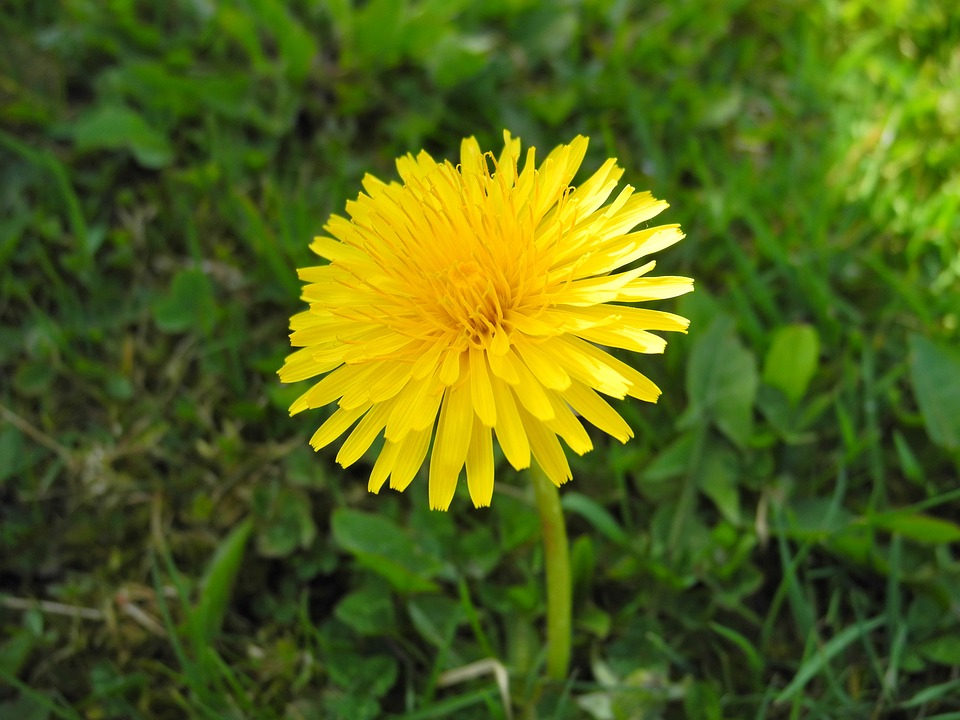
\includegraphics[width=30mm, height=15mm]{images/yellow-18416_960_720-86181412.jpg} & 0.9737037 & xx \\ 
& 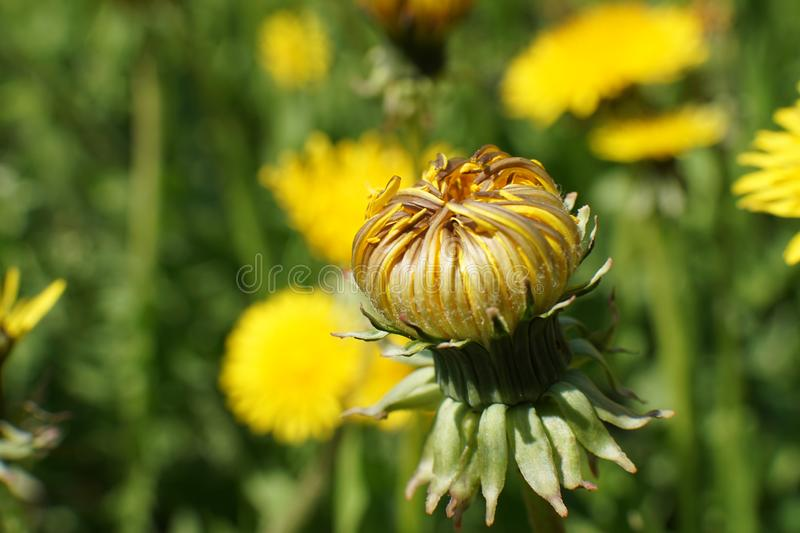
\includegraphics[width=30mm, height=15mm]{images/yellow-dandelion-flowers-taraxacum-officinale-spring-sunny-day-blooming-dandelions-field-background-147943753-1959055877.jpg} & 0.9855896 & xx \\ 
\hline
\end{tabular}
\end{center}
\begin{center}
Table 2. Dandelion Image Accuracy Before and After Attacks
\end{center}
\subsubsection{Correctness}
An adversarial attack deliberate method of manipulating an image to deceive the predictions of a machine learning model. The effectiveness of an attack is measured by its ability to mislead the model while also maintaining the visual appearance of the original image. In the table provided, the accuracy of the model in predicting whether an image depicts grass or dandelions was significantly reduced after applying various adversarial attack algorithms, including genetic algorithm, particle swarm optimization, simulated annealing, hill climbing, and fast gradient sign method. Prior to the attack, the model demonstrated excellent accuracy with a minimum prediction accuracy of 96\% for all images except one. The decrease in accuracy shown by the model after the application of adversarial attacks demonstrates the effectiveness of  the algorithms we chose to use and also potential threats attackers can take advantage of when trying to compromise the performance of a machine learning model.
\subsubsection{Verification}
Verification is the process of checking whether the attack algorithm meets the specifications or requirements. Here we discuss how we would verify the five sub-algorithms that are weighted and combined into one main adversarial attack on the provided grass/dandelion classifier to fool it into incorrectly classifying the image by under 50\%. The tool we would use to verify the code is a static analysis. A static analysis of the algorithm is a method of verifying code correctness by analyzing the code without running it. The tool we would have used is the Lintr package on R. "Lint, or linting, is a tool that analyses source code to flag programming errors, bugs, stylistic errors, and suspicious constructs" (Nicholls, 2023). The package will check for and report syntax errors and possible semantic issues. We found this would be helpful when detecting vulnerabilities/weaknesses in our code.  

\subsection{Runtime,
Complexity, and Walltime}

\subsubsection{Runtime}

\subsubsection{Complexity}
The complexity of adversarial attacks refers to the degree of computational resources, time, and effort needed to create adversarial examples that can effectively deceive machine learning models. It measures the difficulty of performing an attack and the computational power required to produce effective adversarial examples. Our adversarial attack algorithm that utilizes genetic algorithm, particle swarm optimization, simulated annealing, hill climbing, and fast gradient sign method exhibits a high level of complexity due to its iterative nature and large number of possible solutions. While genetic algorithm and particle swarm optimization are computationally expensive since they evaluate each pixel of an image to find the optimal solution, simulated annealing and hill climbing methods are less complex as they focus on evaluating neighboring solutions to identify the most effective one. The fast gradient sign method, on the other hand, is relatively simpler but still involves computing gradients and applying small perturbations to the input image. Overall, the use of these algorithms can be computationally demanding, and therefore it requires us to strike a balance between the complexity and effectiveness of each method.
\subsubsection{Walltime}

The walltime of the algorithm refers to the actual time elapsed from the start to the end of the algorithm execution (Kuo, 2020). Walltime is an important performance metric for adversarial attack algorithms because it is a big factor when determining the practicality of an attack especially in real-time or time-sensitive applications. The walltime is effected by the implementation of the algorithm, which computational resources are used and the complexity of the targeted neural network. The walltime of our algorithm ended up being XXX. We interpreted this as fairly good for the size of the neural network and purpose of the attack.  
\subsection{Performance}
Justifying efficiency trade-offs in light of performance is crucial,
so make sure you document all iterations of your algorithm and why you took that specific development path. 

We used the following scoring equation, $\sum_{b=1}^{0.01*P} f * \frac{P}{b}$, where P is the number of pixels in the image and f is the number of successfully fooled images at a given budget level b, to determine our algorithm performance. 

%REFERENCES
\newpage
\section{References}
\begin{thebibliography}{9}

\bibitem{Abbas}
Abbas, A. K. (2011). Fuzzy logic control in support of autonomous navigation of humanitarian de-mining robots. Elsevier EBooks, 453–475. https://doi.org/10.1533/9780857090201.4.453

\bibitem{ansah}
Ansah, H. (2022, July 21). Adversarial Attacks on Neural Networks: Exploring the Fast Gradient Sign Method - neptune.ai. Neptune.ai. https://neptune.ai/blog/adversarial-attacks-on-neural-networks-exploring-the-fast-gradient-sign-method

\bibitem{balda2019adversarial}
Balda, E. R., Behboodi, A., \& Mathar, R. (2019). Adversarial examples in deep neural networks: An overview. Deep Learning: Algorithms and Applications, 31–65. https://doi.org/10.1007/978-3-030-31760-7\_2

\bibitem{brownlee2021simulated}
Brownlee, J. (2021, October 11). Simulated annealing from scratch in Python. Machine Learning Mastery. Retrieved April 23, 2023, from https://machinelearningmastery.com/simulated-annealing-from-scratch-in-python/

\bibitem{carlini2017towards}
Carlini, N., \& Wagner, D. (2017). Towards evaluating the robustness of neural networks. 2017 IEEE Symposium on Security and Privacy (SP). https://doi.org/10.1109/sp.2017.49

\bibitem{goodfellow2015explaining}
Goodfellow, I. J., Shlens, J., \& Szegedy, C. (2015). Explaining and Harnessing Adversarial Examples. ICLR. https://doi.org/arXiv:1412.6572v3

\bibitem{kuowalltime}
Kuo, Y.-C. (2021, December 9). ML09: Measuring running time in Python \& R. Medium. Retrieved April 25, 2023, from https://yc-kuo.medium.com/ml09-e549b2c26c47 

\bibitem{mallawaarachchi2020introduction}
Mallawaarachchi, V. (2020, March 1). Introduction to genetic algorithms. Medium. Retrieved April 23, 2023, from https://towardsdatascience.com/introduction-to-genetic-algorithms-including-example-code-e396e98d8bf3

\bibitem{nicholls2023linting}
Nicholls, R. (2023). Introduction to R:linting R (and R markdown). Introduction to R: Linting R (and R Markdown). Retrieved April 24, 2023, from https://rowannicholls.github.io/R/intro/linting.html 

\bibitem{tyshevskyi2019adversarial}
Pavel Tyshevskyi. (2019, September 28). Adversarial Attack Using Genetic Algorithm - Analytics Vidhya - Medium. Medium; Analytics Vidhya. https://medium.com/analytics-vidhya/adversarial-attack-using-genetic-algorithm-90beba13b6cb

\bibitem{ren2020adversarial}
Ren, K., Zheng, T., Qin, Z., \& Liu, X. (2020). Adversarial attacks and defenses in Deep Learning. Engineering, 6(3), 346–360. https://doi.org/10.1016/j.eng.2019.12.012

\bibitem{kukovec2021adversarial}
Rok Kukovec, Pecnk, S., Iztok Fister jr, \& Sašo Karakatič. (2021, September 13). Adversarial Image Perturbation with a Genetic Algorithm. ResearchGate; unknown. https://www.researchgate.net/publication/354557862\_Adversarial\_Image\_Pertubation\_with\_a\_Genertic\_\\Algorithm

\bibitem{tam2021gentle}
Tam, A. (2021, October 11). A gentle introduction to particle swarm optimization. Machine Learning Mastery. Retrieved April 23, 2023, from https://machinelearningmastery.com/a-gentle-introduction-to-particle-swarm-optimization/

‌\bibitem{tsui}
Tsui, K. (2018, August 20). Perhaps the Simplest Introduction of Adversarial Examples Ever. Medium; Towards Data Science. https://towardsdatascience.com/perhaps-the-simplest-introduction-of-adversarial-examples-ever-c0839a759b8d

\bibitem{visiblebreadcrumbs}
VisibleBreadcrumbs. (2023). Mathworks.com. https://www.mathworks.com/help/gads/what-is-particle-swarm-optimization.html

\bibitem{wang}
Wang, D., Tan, D., Liu, \& Liu, L. (n.d.). Particle swarm optimization algorithm: an overview. https://kpfu.ru/staff\_files/F\_1407356997/overview.pdf
‌
\end{thebibliography}
\end{document}
